% ============================================================================
% Networks Decide for Us — CPIN 2026 (Critical Phenomena in Networks)
% Style replicates the "JORNADA REDES" deck: white background, centered frame
% titles with a red rule, dark-red accents, green reference markers, LaTeX math.
% Compile: pdflatex presentation-cpin2.tex  (run twice)
% ============================================================================
\documentclass[aspectratio=169,11pt]{beamer}

\usepackage[utf8]{inputenc}
\usepackage[T1]{fontenc}
\usepackage{amsmath, amssymb}
\usepackage{graphicx}
\usepackage{booktabs}
\usepackage{array}
\usepackage{xcolor}
\usepackage{tikz}
\usepackage{qrcode}
\usetikzlibrary{arrows.meta, positioning, calc}

% ---------- Fonts: clean humanist sans, professional math ----------
\usefonttheme{professionalfonts}
\usepackage{helvet}
\renewcommand{\familydefault}{\sfdefault}

% ---------- Colors (matched to the JORNADA deck) ----------
\definecolor{ndred}{RGB}{222,32,38}       % bright red rule
\definecolor{ndreddark}{RGB}{176,22,28}   % darker brick red (subtitles)
\definecolor{ndgreen}{RGB}{0,164,80}      % green reference markers
\definecolor{ndblue}{RGB}{30,90,200}      % path-1 blue
\definecolor{ndgray}{RGB}{90,90,90}

% ---------- Strip all Beamer chrome ----------
\setbeamertemplate{navigation symbols}{}
\setbeamercolor{normal text}{fg=black,bg=white}
\setbeamercolor{structure}{fg=ndreddark}
\setbeamertemplate{itemize item}{\color{ndreddark}\textbullet}
\setbeamertemplate{itemize subitem}{\color{ndgray}\textendash}

% ---------- Frame title: centered black title + full-width red rule ----------
\setbeamercolor{frametitle}{fg=black,bg=white}
\setbeamerfont{frametitle}{size=\Large, series=\mdseries}
\setbeamertemplate{frametitle}{%
  \vspace{0.35cm}%
  \begin{center}\insertframetitle\end{center}%
  \vspace{-0.18cm}%
  {\color{ndred}\hrule height 1.1pt}%
}

% ---------- Minimal footline: page number only ----------
\setbeamertemplate{footline}{%
  \hfill{\color{ndgray}\scriptsize\insertframenumber}\hspace{0.5cm}\vspace{0.2cm}}

% ---------- Helper macros ----------
\newcommand{\refn}[1]{{\color{ndgreen}[#1]}}
\newcommand{\emphr}[1]{{\color{ndreddark}\textbf{#1}}}

% Section-divider slide: centered title with a short red underline
\newcommand{\sectionslide}[1]{%
  \begin{frame}[plain]
    \vfill
    \begin{center}
      {\Large #1}\\[2pt]
      {\color{ndred}\rule{0.30\textwidth}{1.1pt}}
    \end{center}
    \vfill
  \end{frame}}

% Six-node network snapshot. Args = fill colour (black/white) for nodes 1..6.
% Shared topology: hub node 4; edges 1-4, 2-4, 4-6, 4-5, 1-2; node 3 isolated.
\newcommand{\sixnet}[6]{%
\begin{tikzpicture}[scale=0.5,baseline=-0.6cm]
  \coordinate (a1) at (0,1.0);   \coordinate (a2) at (-1.05,0.05);
  \coordinate (a3) at (2.0,1.0); \coordinate (a4) at (1.0,0);
  \coordinate (a5) at (0.25,-1.1);\coordinate (a6) at (2.35,-0.35);
  \draw[gray] (a1)--(a4) (a2)--(a4) (a4)--(a6) (a4)--(a5) (a1)--(a2);
  \foreach \p/\c/\n in {a1/#1/1,a2/#2/2,a3/#3/3,a4/#4/4,a5/#5/5,a6/#6/6}
    \node[circle,draw,fill=\c,minimum size=4.6mm,inner sep=0pt,
          label={[font=\tiny,text=ndgray,inner sep=1pt]above:\n}] at (\p){};
\end{tikzpicture}}
\newcommand{\snaparrow}{\ {\color{ndred}\large$\boldsymbol{\Rightarrow}$}\ }

% ============================================================================
\title{Networks Decide for Us}
\subtitle{When homophily governs the criticality of social adoption}
\author{Aníbal Olivera M.}
\date{}

\begin{document}

% ---------------------------------------------------------------- TITLE
\begin{frame}[plain]
  \vspace{0.6cm}
  \begin{center}
    {\footnotesize\color{ndgray} Centro de Investigación en Complejidad Social (CICS) $\cdot$ Universidad del Desarrollo}
  \end{center}
  \vspace{1.1cm}
  \begin{center}
    {\LARGE \textbf{Networks Decide for Us}}\\[0.5cm]
    {\large \color{ndreddark} When homophily governs the criticality of social adoption}
  \end{center}
  \vspace{1.4cm}
  \begin{center}
    {\normalsize Aníbal Olivera M.}\\[2pt]
    {\footnotesize PhD(c) in Social Complexity Sciences, CICS}\\[2pt]
    {\footnotesize with Jorge Fábrega \& Thomas W. Valente}
  \end{center}
  \vfill
  \begin{center}
    {\scriptsize\color{ndgray} Critical Phenomena in Networks (CPIN) — 2026}
  \end{center}
\end{frame}

% ---------------------------------------------------------------- OVERVIEW
\begin{frame}{The question}
\begin{itemize}
  \item Collective behaviors (innovations, mobilizations) spread as \emphr{adoption cascades} on social networks.
  \vspace{0.3cm}
  \item Most models use \emph{synthetic} topologies and treat agents as cognition-free relays \refn{1}.
  \vspace{0.3cm}
  \item Real networks are shaped by \emphr{multidimensional homophily} — similar people cluster \refn{2}.
\end{itemize}
\vspace{0.5cm}
\begin{center}
\fcolorbox{ndred}{white}{\parbox{0.9\textwidth}{\centering
Conditional on \emph{fixed individual propensities}, can the \emphr{shape of more realistic
networks alone} change the outcome? Can the structure itself be an \emphr{autonomous force},
deciding not just \emph{how much} spreads, but \emph{how} it spreads?}}
\end{center}
\end{frame}

% ================================================================ THE MODEL
\sectionslide{The model}

% ---- Rational choice  (point 1: separated IUL/MUR ; point 2: 3 rational snapshots)
\begin{frame}{The model — 1) Rational Choice}
\begin{itemize}
  \item Following the literature, the attractiveness of the innovation is its
        \emph{Intrinsic Utility Level} (IUL), $\Gamma\in[0,1]$.
  \item Each person has a \emph{Minimum Utility Requirement} (MUR), $q_i\in[0,1]$,
        representing their aversion to adopting the behavior.
\end{itemize}
\vspace{0.15cm}
\begin{center}
An agent adopts on its own iff\quad
\fcolorbox{ndred}{white}{$\;q_i \le \Gamma \;\implies\; a_i = 1\;$}
\end{center}
\vspace{0.25cm}
\begin{center}
\sixnet{black}{white}{white}{white}{white}{white}\snaparrow
\sixnet{black}{white}{white}{black}{white}{white}\snaparrow
\sixnet{black}{black}{white}{black}{white}{black}
\end{center}
\begin{center}\footnotesize
Everyone with $q_i\le\Gamma$ adopts, regardless of neighbors:
\emphr{deterministic} and \emphr{topology-blind}.
\end{center}
\end{frame}

% ---- Selective social influence (point 2: 3 social snapshots)
\begin{frame}{The model — 2) Selective Social Influence}
If intrinsic adoption fails, an agent may still adopt by peer contagion if
$\tau_i \le \tilde{E}_i$ \refn{5,6} — but only \emph{influential} peers, those socially
\emph{close} in Blau space \refn{7}, count:
\begin{equation*}\small
  \tilde{E}_i \equiv \frac{\sum_{j\neq i}\mathbf{X}_{ij}\,\tilde{a}_j}{\sum_{j\neq i}\mathbf{X}_{ij}},
  \qquad
  \tilde{a}_j = 1 \iff a_j = 1 \;\wedge\; U_{ij} \le \sigma\!\left(MSP - d_{ij}\right)
\end{equation*}
\vspace{-0.15cm}
\begin{center}
\sixnet{black}{white}{white}{white}{black}{white}\snaparrow
\sixnet{black}{black}{white}{white}{black}{white}\snaparrow
\sixnet{black}{black}{white}{black}{black}{white}
\end{center}
\begin{center}\footnotesize
$\tau_4=0.5$: close adopters $d_{14},d_{24}<MSP$ count; the distant one $d_{54}>MSP$ does
\emph{not} $\Rightarrow$ node 4 ignites from similar peers only.\\
\emphr{MSP} (Maximum Social Proximity) sets how far influence reaches; this channel is
\emphr{stochastic} and \emphr{topology-sensitive}.
\end{center}
\end{frame}

% ================================================================ SETTING UP
\sectionslide{Imputing structure \& running the model}

% ---- Imputation slide (points 4,5: horizontal pipeline, image bottom-right)
\begin{frame}{Imputing a network onto a survey}
\begin{center}
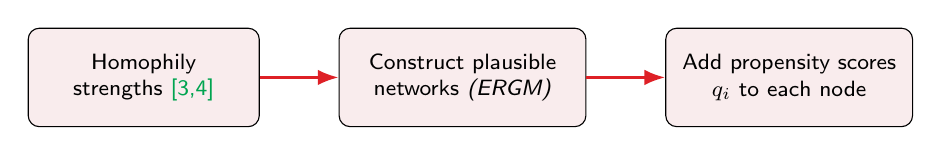
\begin{tikzpicture}[every node/.style={font=\footnotesize}]
  \node[draw,rounded corners,fill=ndreddark!8,text width=2.7cm,align=center,
        minimum height=1.25cm] (a) {Homophily strengths \refn{3,4}};
  \node[draw,rounded corners,fill=ndreddark!8,text width=2.9cm,align=center,
        minimum height=1.25cm,right=1.0cm of a] (b) {Construct plausible networks \emph{(ERGM)}};
  \node[draw,rounded corners,fill=ndreddark!8,text width=2.9cm,align=center,
        minimum height=1.25cm,right=1.0cm of b] (c) {Add propensity scores $q_i$ to each node};
  \draw[-{Latex},ndred,line width=1pt] (a)--(b);
  \draw[-{Latex},ndred,line width=1pt] (b)--(c);
\end{tikzpicture}
\end{center}
\vspace{0.2cm}
\begin{columns}[c]
\column{0.52\textwidth}
\footnotesize
Tie probability is a function of distance in Blau space (age, sex, education, race, religion):
\begin{equation*}\footnotesize
  \mathrm{logit}\,\Pr(Y_{ij}=1)=\alpha+\boldsymbol\beta^\top \mathbf{d}_{ij}
\end{equation*}
$\hat{\boldsymbol\beta}$ comes from GSS confidant data \refn{4}; propensities $q_i$ come from
real survey answers (innovation, collective action).
\column{0.48\textwidth}
\centering
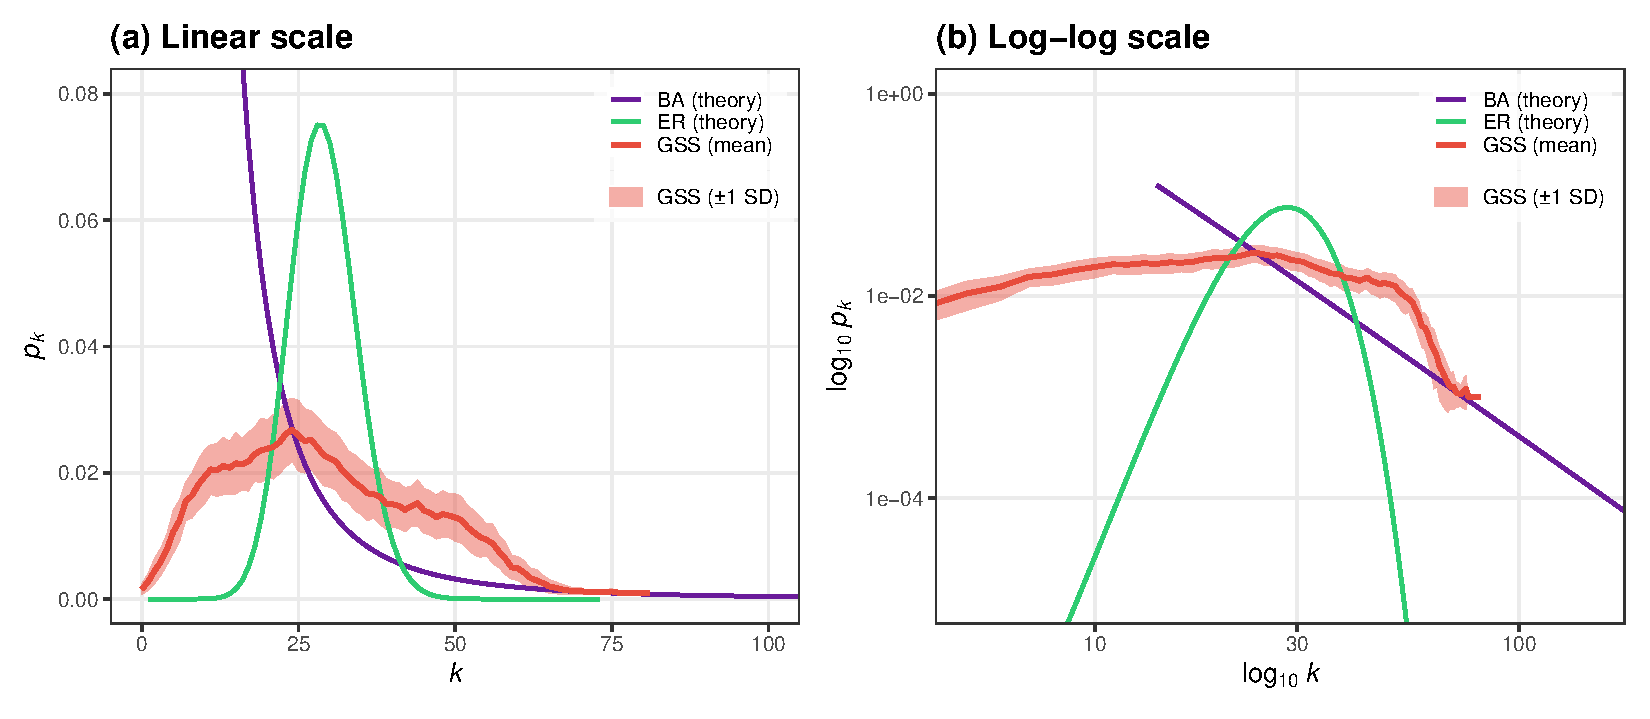
\includegraphics[width=0.92\linewidth]{../../plots/02_GSS_network_ergm_tests/GSS_degree_dist.pdf}\\
{\scriptsize Right-skewed degree structure that ER / BA models fail to match jointly.}
\end{columns}
\end{frame}

\begin{frame}{Comprehensive simulation design}
Hybrid social contagion via \texttt{netdiffuseR} \refn{9}, over plausible (GSS) vs.\
\emphr{degree-preserving randomized} (GSS-DP) topologies.
\vspace{0.2cm}
\begin{itemize}
  \item \textbf{IUL} ($\Gamma$): 41 levels $[0,1]$. \quad \textbf{MSP} ($h$): 13 levels $[0,1]$.
  \item \textbf{Thresholds} $\tau_i\sim\mathcal{N}(\mu,\sigma)$: $\mu\in\{.3,.4,.5,.6\}$, $\sigma\in\{.08,.12,.16,.20\}$.
  \item \textbf{Seeding}: random, central, marginal, closeness, eigenvector.
\end{itemize}
\vspace{0.2cm}
\begin{center}
Total: $\;41\times13\times4\times4\times5\times \text{(runs)} \;\approx\; \emphr{$4\times10^{6}$ simulations}$
\end{center}
\vspace{0.2cm}
We then fit \emph{Big Additive Models} (BAM) to isolate the structural effect:
\begin{equation*}\footnotesize
  \mathrm{logit}\big[\mathbb{E}(\Phi)\big]=\beta_0+\mathbf{Z}\boldsymbol\beta
  +\beta_{\text{DP}}\,\mathbb{I}_{\text{DP}}+s(\mathrm{IUL},\mathrm{MSP})
\end{equation*}
\end{frame}

% ================================================================ PHYSICS MAP
\sectionslide{A statistical-physics reading}

\begin{frame}{Mapping social adoption to a ferromagnet}
\begin{columns}[c]
\column{0.56\textwidth}
\renewcommand{\arraystretch}{1.35}
\begin{tabular}{@{}l@{\;\;}c@{\;\;}l@{}}
\toprule
\textbf{Ising system} & & \textbf{NDFU} \\
\midrule
Spin $s_i\in\{0,1\}$        & $\leftrightarrow$ & Adoption state $a_i$ \\
Magnetization $M$           & $\leftrightarrow$ & Adoption $\Phi=N_{\text{ad}}/N$ \\
External field $H$          & $\leftrightarrow$ & \emphr{IUL} $\Gamma$ (rational bias) \\
Temperature $T$             & $\leftrightarrow$ & \emphr{MSP} $h$ (social agitation) \\
Exchange $J_{ij}$           & $\leftrightarrow$ & Homophily / clustering \\
Susceptibility $\chi$       & $\leftrightarrow$ & $\mathrm{Var}(\Phi)$ (FDT) \\
\bottomrule
\end{tabular}
\column{0.44\textwidth}
\footnotesize
Pseudo-Hamiltonian:
\begin{equation*}
\mathcal{H}\approx -\!\!\sum_{\langle i,j\rangle}\! w_{ij}(h)\,s_i s_j \;-\; \Gamma\sum_i s_i
\end{equation*}
\vspace{0.1cm}
\emphr{Low MSP} $\to$ rigid echo chambers (frozen domains).\\[3pt]
\emphr{High MSP} $\to$ boundaries ``melt'', global cascades possible.
\end{columns}
\vspace{0.3cm}
\begin{center}\footnotesize
Susceptibility diverges near criticality \refn{8}: $\;\chi=\mathrm{Var}(\Phi)\propto |MSP-MSP_c|^{-\gamma}$
\end{center}
\end{frame}

% ---- Two paths slide (point 10: cleaner 3D depth ; point 8: asymmetry framing)
\begin{frame}{Two paths through the critical point}
\begin{columns}[c]
\column{0.52\textwidth}
\centering
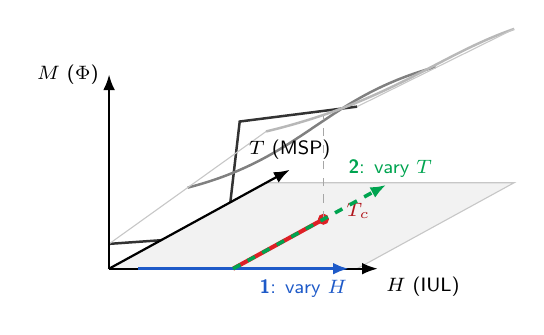
\begin{tikzpicture}[scale=1.05, font=\scriptsize, >={Latex[length=2mm]}]
  \def\px{0.95}\def\py{0.52}                 % depth (T) step
  % ---- response surface M(T,H): 3 waterfall profiles, front=sharp, back=smooth ----
  \foreach \i/\op in {0/80,1/50,2/28}{
    \begin{scope}[shift={(\i*\px,\i*\py)}]
      \ifnum\i=0
        \draw[black!\op,line width=0.9pt] (0,0.30)--(1.42,0.40)--(1.58,1.78)--(3,1.96);
      \else\ifnum\i=1
        \draw[black!\op,line width=0.9pt] (0,0.46) .. controls (1.4,0.82) and (1.65,1.55) .. (3,1.92);
      \else
        \draw[black!\op,line width=0.9pt] (0,0.62) .. controls (1.5,0.98) and (2.1,1.55) .. (3,1.86);
      \fi\fi
    \end{scope}
  }
  \draw[black!22] (0,0.30)--(2*\px,0.62+2*\py);     % sheet side rails
  \draw[black!22] (3,1.96)--(3+2*\px,1.86+2*\py);
  % ---- floor (T,H) control plane at M=0 ----
  \fill[black!5] (0,0)--(3,0)--(3+2*\px,2*\py)--(2*\px,2*\py)--cycle;
  \draw[black!22] (0,0)--(3,0)--(3+2*\px,2*\py)--(2*\px,2*\py)--cycle;
  % axes
  \draw[->,thick] (0,0)--(3.25,0) node[below right=-1pt]{$H$ (IUL)};
  \draw[->,thick] (0,0)--($(2*\px,2*\py)+(0.3*\px,0.3*\py)$) node[above]{$T$ (MSP)};
  \draw[->,thick] (0,0)--(0,2.35) node[left]{$M$ ($\Phi$)};
  % first-order coexistence line (on floor) ending at the critical point
  \coordinate (cp) at ($(1.5,0)+(1.15*\px,1.15*\py)$);
  \draw[ndred,line width=1.5pt] (1.5,0)--(cp);
  \filldraw[ndred] (cp) circle (1.7pt);
  \node[ndreddark] at ($(cp)+(0.42,0.10)$){$T_c$};
  \draw[black!35,dashed] (cp)--($(cp)+(0,1.25)$);    % tie floor point to surface kink
  % Path 1 (blue): vary H at fixed (low) T — crosses the coexistence line
  \draw[ndblue,line width=1.3pt,->] (0.35,0)--(2.9,0);
  \node[ndblue] at (2.35,-0.24){\textbf{1}: vary $H$};
  % Path 2 (green): vary T at fixed H — runs into the critical point
  \draw[ndgreen,line width=1.3pt,dashed,->] (1.5,0)--($(1.5,0)+(1.95*\px,1.95*\py)$);
  \node[ndgreen] at ($(1.5,0)+(1.95*\px,1.95*\py)+(0.05,0.2)$){\textbf{2}: vary $T$};
\end{tikzpicture}
\column{0.48\textwidth}
\footnotesize
\textbf{\color{ndgreen}Path 2 — vary MSP ($T$) at fixed IUL}
\begin{itemize}\footnotesize
  \item continuous \emphr{2nd-order} transition; exponent $\gamma$
  \item drives the \emphr{social channel} $\Rightarrow$ \emphr{topology-sensitive}
  \item \emphr{only the plausible network reaches $\gamma\approx1$}
\end{itemize}
\vspace{0.2cm}
\textbf{\color{ndblue}Path 1 — vary IUL ($H$) at fixed MSP}
\begin{itemize}\footnotesize
  \item field-direction response; exponent $\delta$
  \item drives the \emphr{rational channel} $\Rightarrow$ \emphr{topology-blind}
  \item \emphr{both} networks give the same $\delta\approx3$
\end{itemize}
\end{columns}
\end{frame}

% ================================================================ RESULTS
\sectionslide{Results}

% ---- Result 1 = DYNAMICS (point 12 reorder)
\begin{frame}{Result 1 — Criticality signatures (dynamics)}
\centering
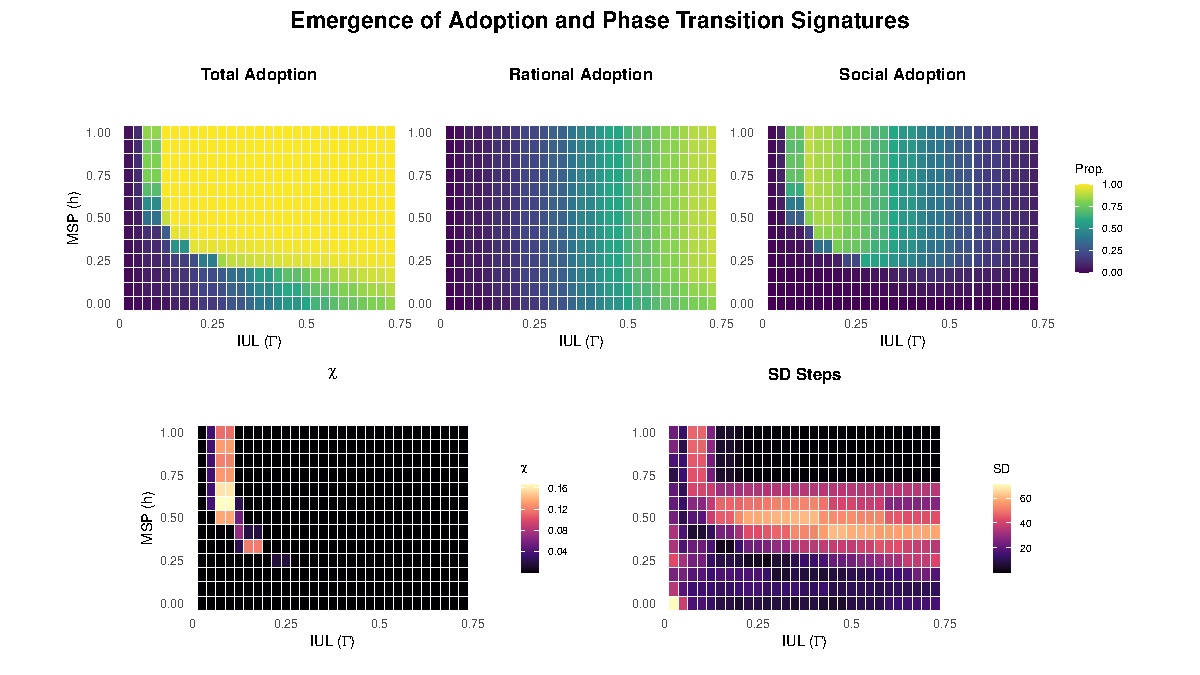
\includegraphics[width=0.98\textwidth]{../abstract-sn26/figure1_5panels_GSS.pdf}\\[2pt]
{\footnotesize Top: Total, Rational and Social adoption. Rational adoption grows smoothly with
IUL; \emph{social} adoption is more complex, keeping total adoption high over a wide region.
Bottom-left: susceptibility $\chi=\mathrm{Var}(\Phi)$ ridge; bottom-right: relaxation-time SD
divergence — \emphr{Critical Slowing Down}.}
\end{frame}

% ---- Result 2 = STRUCTURAL PREMIUM (point 11: full OR table)
\begin{frame}{Result 2 — A structural premium (volume)}
\begin{columns}[c]
\column{0.46\textwidth}
BAM isolates the marginal effect of destroying empirical structure:
\vspace{0.2cm}
\begin{center}
\fcolorbox{ndred}{white}{$\;\beta_{\text{DP}}=-0.850^{***}\;$ (OR $=0.43$)}\\[4pt]
{\footnotesize $\Rightarrow$ randomization cuts adoption odds by $\sim$\emphr{57\%}}
\end{center}
\vspace{0.2cm}
\footnotesize Under \emph{identical} propensities, homophilic clustering lets social
reinforcement build inside \emphr{local echo chambers} — even for unattractive
innovations ($\Gamma<0.25$).
\column{0.54\textwidth}
\centering
\renewcommand{\arraystretch}{1.12}
{\scriptsize
\begin{tabular}{@{}lcc@{}}
\toprule
\textbf{Total adoption (GSS)} & Estimate & OR \\
\midrule
(Intercept) & $6.534^{***}$ & --- \\
$\tau_{\text{mean}}$ & $-6.944^{***}$ & --- \\
$\tau_{\text{sd}}$ & $5.942^{***}$ & --- \\
\addlinespace
\multicolumn{3}{@{}l}{\textit{Seeding (ref: Random)}}\\
\quad Central & $0.120^{***}$ & 1.127 \\
\quad Closeness & $0.119^{***}$ & 1.126 \\
\quad Eigenvector & $0.118^{***}$ & 1.125 \\
\quad Marginal & $-0.067^{***}$ & 0.935 \\
\addlinespace
\multicolumn{3}{@{}l}{\textit{Topology (ref: Plausible)}}\\
\quad Deg.-pres. random & $\mathbf{-0.850}^{***}$ & \textbf{0.427} \\
\midrule
\multicolumn{3}{@{}l}{Deviance explained: 82.2\%\quad $N=4{,}093{,}440$}\\
\bottomrule
\end{tabular}}
\\[3pt]{\scriptsize $^{***}p<0.001$. OR $=\exp(\beta)$.}
\end{columns}
\end{frame}

% ---- Result 3 = UNIVERSALITY (point 8 reframe ; point 15 fixed table)
\begin{frame}{Result 3 — Universality is exclusive to plausible networks}
\begin{columns}[c]
\column{0.5\textwidth}
\centering
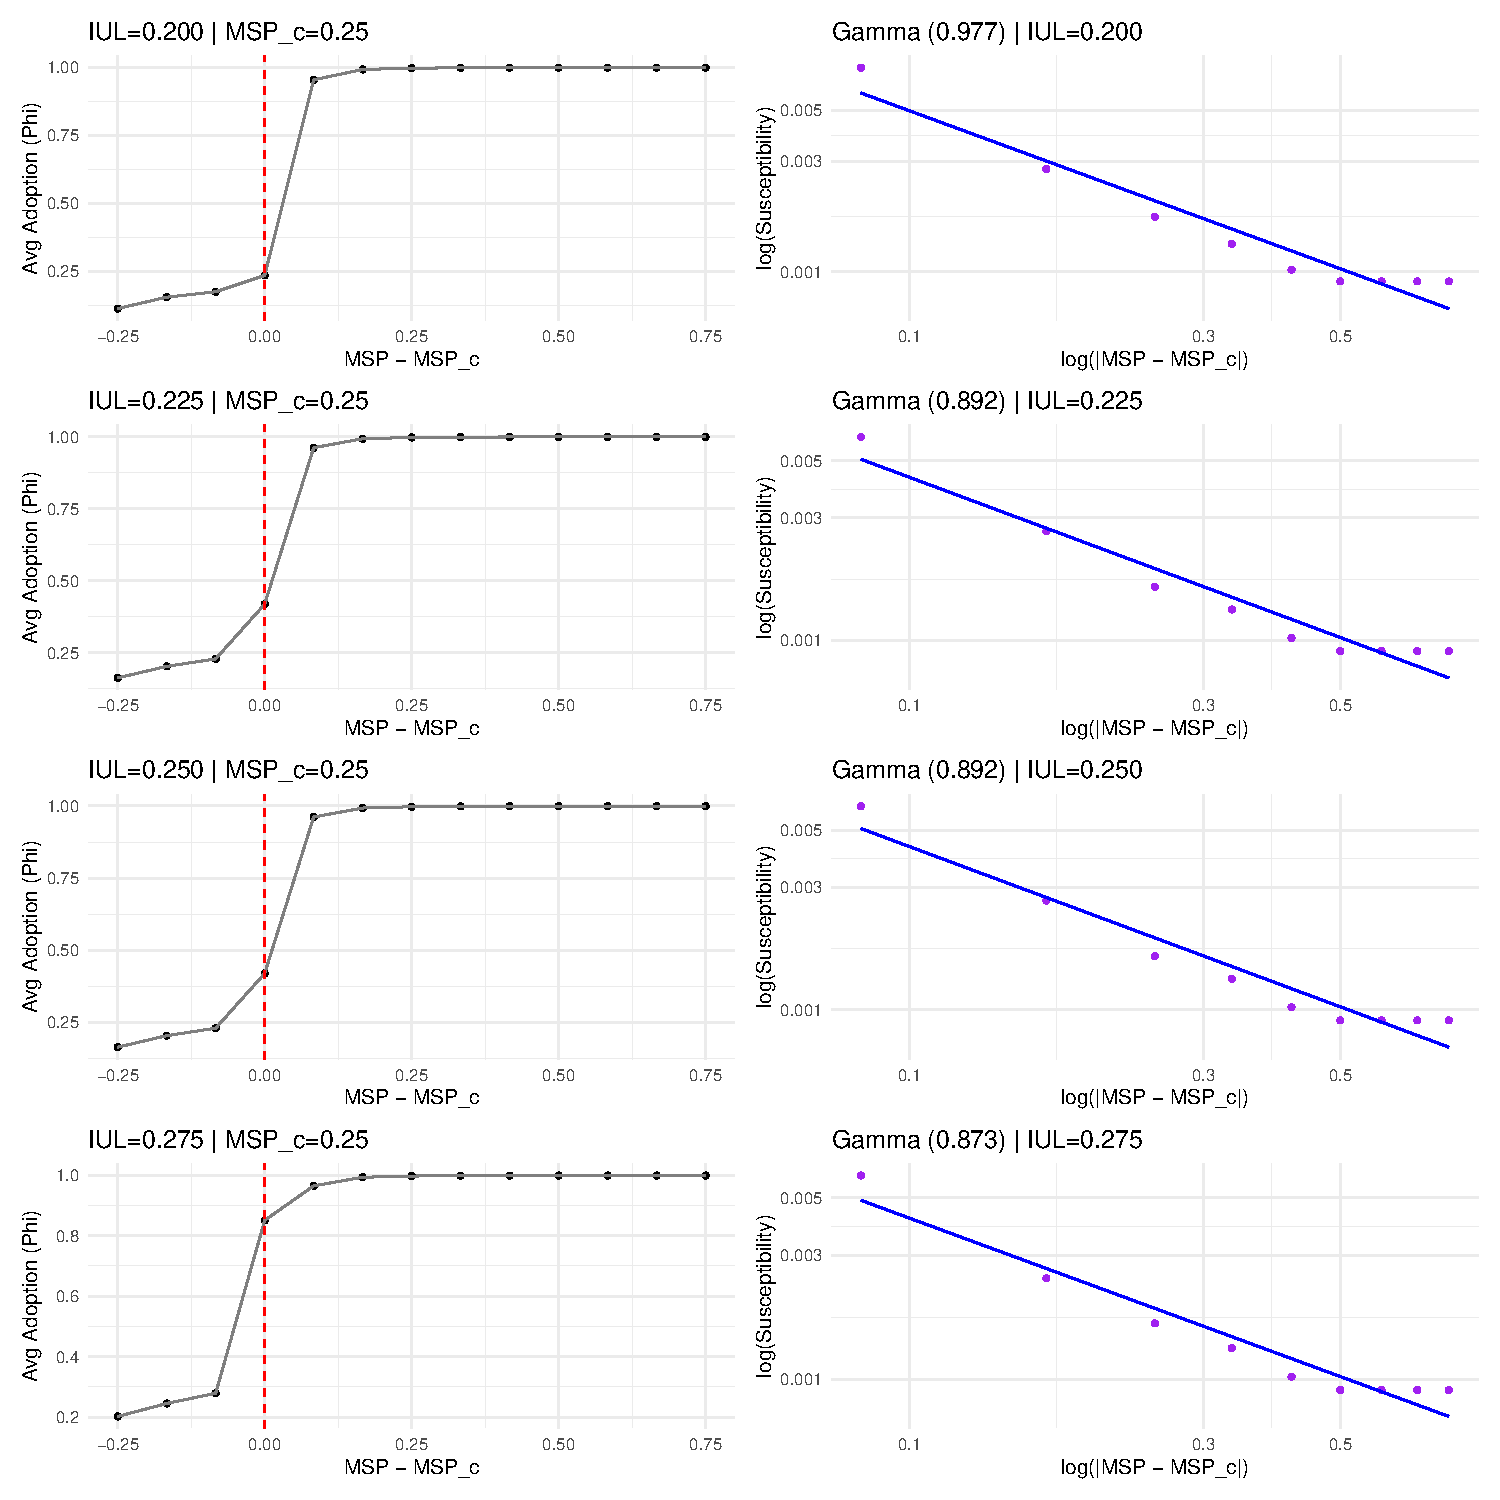
\includegraphics[width=\linewidth]{../../plots/07_phase_transition/GSS/method4_exponents.pdf}\\
{\scriptsize Log-log: $\chi\sim|MSP-MSP_c|^{-\gamma}$ along the Widom line.}
\column{0.5\textwidth}
\renewcommand{\arraystretch}{1.25}
{\footnotesize
\begin{tabular}{@{}lcc@{}}
\toprule
IUL & Plausible $\gamma$ & Randomized $\gamma$ \\
\midrule
0.200 & 0.98 & 3.71 \\
0.225 & 0.89 & 3.67 \\
0.250 & 0.89 & 3.67 \\
0.275 & 0.87 & 4.67 \\
\midrule
mean & \emphr{0.91} & \emphr{3.93} \\
\bottomrule
\end{tabular}}
\vspace{0.15cm}
\begin{itemize}\scriptsize
  \item \emphr{Only} the plausible (homophilic) network reaches $\gamma\approx1$ —
        \emph{Mean-Field universality}, a continuous transition.
  \item Randomization $\Rightarrow\gamma\approx4$: no power law, \emphr{discontinuous} regime shift.
  \item Separation $\approx\mathbf{4.3\times}$.
\end{itemize}
\end{columns}
\end{frame}

\begin{frame}{Why only the MSP axis discriminates}
\begin{columns}[c]
\column{0.52\textwidth}
\textbf{Two control parameters, two channels:}
\begin{itemize}\footnotesize
  \item \emphr{Path 2 (MSP, $\gamma$)}: the \emph{social} channel.
        $\gamma_{\text{GSS}}\!\approx\!1$ vs.\ $\gamma_{\text{DP}}\!\approx\!4$ — \emphr{discriminates}.
  \item \emphr{Path 1 (IUL, $\delta$)}: the \emph{rational} channel ($q_i\le\Gamma$ is node-local).
        $\delta_{\text{GSS}}\!\approx\!2.85$, $\delta_{\text{DP}}\!\approx\!2.91$ — \emphr{both $\approx$ MF $\delta=3$}.
\end{itemize}
\vspace{0.2cm}
\footnotesize The field response reflects the \emph{MUR distribution}, shared by both topologies.
So ``universality'' is \emphr{not} generic — it is a fingerprint of empirically homophilic structure.
\column{0.48\textwidth}
\centering
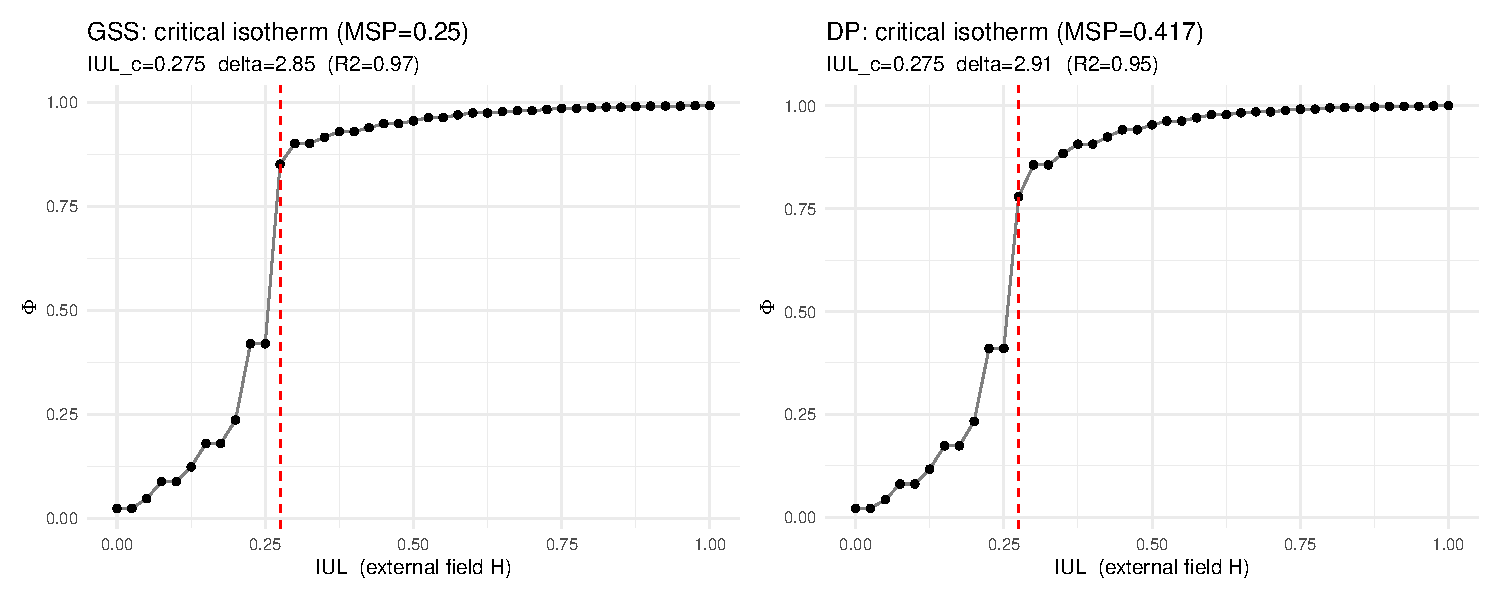
\includegraphics[width=\linewidth]{../../playground/checks-claude/plots/camino_H_critical_isotherm.pdf}\\
{\scriptsize Critical isotherms $\Phi(\mathrm{IUL})$: same $\delta\!\approx\!3$ for both. \emph{(exploratory)}}
\end{columns}
\end{frame}

% ================================================================ DISCUSSION
\begin{frame}{The mean-field paradox — and its resolution}
\begin{block}{\footnotesize Puzzle}
\footnotesize Mean-field $\gamma=1$ usually needs a \emph{well-mixed} system.
We recover it in a \emph{strongly clustered, homophilic} network.
\end{block}
\vspace{0.1cm}
\begin{block}{\footnotesize Resolution}
\footnotesize Homophilic clusters behave as quasi-isolated subsystems coupled by
\emph{weak, similarity-selective bridges}. As MSP $\to MSP_c$ these bridges activate
together, synchronizing clusters into one coherent order parameter — \emph{indistinguishable}
from mean-field behavior. Randomization (DP) destroys this and yields discontinuity instead.
\end{block}
\vspace{0.1cm}
\begin{center}\footnotesize
Homophily gives the system a \emphr{``sociological viscosity''}: tipping points arrive
\emph{with measurable early warning} (rising variance, slow recovery) instead of detonating blind.
\end{center}
\end{frame}

% ================================================================ CONCLUSION
\sectionslide{Conclusions}

% ---- Conclusions structured as answers to the two opening questions (point 18 + 16)
\begin{frame}{Conclusions}
\begin{center}{\large \emphr{Networks decide for us} — and the answer to both opening questions is \emph{yes}.}\end{center}
\vspace{0.25cm}
\textbf{\color{ndgreen}Q1. Can the shape of realistic networks \emph{alone} change the outcome?}
\begin{itemize}\footnotesize
  \item \emphr{Volume:} empirical homophily yields a \emphr{structural premium} ($+57\%$ odds).
  \item When society is not too restrictive (high MSP), \emphr{highly attractive and unattractive
        innovations reach nearly the same adoption} — purely through social influence.
\end{itemize}
\vspace{0.15cm}
\textbf{\color{ndgreen}Q2. Is structure an autonomous force deciding \emph{how} it spreads?}
\begin{itemize}\footnotesize
  \item \emphr{Dynamics:} homophily makes tipping points \emphr{continuous \& predictable}
        ($\gamma\approx1$); randomization makes them \emphr{abrupt \& volatile} ($\gamma\approx4$).
  \item Universality is \emphr{exclusive} to plausible networks; the rational (IUL) axis is
        topology-blind ($\delta\approx3$).
\end{itemize}
\vspace{0.2cm}
\begin{center}\footnotesize
Macroscopic social change is not the linear sum of individual preferences —
it is governed by the structure of our ties.
\end{center}
\end{frame}

% ---------------------------------------------------------------- REFERENCES
\begin{frame}{References}
\footnotesize
\begin{enumerate}\itemsep1.5pt
  \item Goldberg, A. (2021). Associative Diffusion and the Pitfalls of Structural Reductionism. \emph{Am. Sociol. Rev.} 86(6).
  \item McPherson, M., Smith-Lovin, L., \& Cook, J. (2001). Birds of a Feather: Homophily in Social Networks. \emph{Annu. Rev. Sociol.} 27.
  \item McPherson, M., \& Smith, J. A. (2019). Network Effects in Blau Space: Imputing Social Context from Survey Data. \emph{Socius} 5.
  \item Smith, J. A., McPherson, M., \& Smith-Lovin, L. (2014). Social Distance in the United States, 1985--2004. \emph{Am. Sociol. Rev.} 79(3).
  \item Granovetter, M. (1978). Threshold Models of Collective Behavior. \emph{Am. J. Sociol.} 83(6).
  \item Valente, T. W. (1996). Social Network Thresholds in the Diffusion of Innovations. \emph{Soc. Networks} 18(1).
  \item Centola, D. (2011). An Experimental Study of Homophily in the Adoption of Health Behavior. \emph{Science} 334.
  \item Sethna, J. P. (2021). \emph{Statistical Mechanics: Entropy, Order Parameters, and Complexity} (2nd ed.). Oxford UP.
  \item Vega Yon, G., Olivera M., A., \& Valente, T. (2025). \texttt{netdiffuseR}: Analysis of Diffusion and Contagion Processes on Networks. \emph{Zenodo}.
\end{enumerate}
\end{frame}

% ---------------------------------------------------------------- THANKS (point 17: QR)
\begin{frame}[plain]
  \vfill
  \begin{center}
    {\Large Thanks!}\\[2pt]
    {\color{ndred}\rule{0.30\textwidth}{1.1pt}}\\[0.7cm]
    \qrcode[height=2.3cm]{https://github.com/aoliveram/Networks-Decide-for-Us}\\[0.35cm]
    {\footnotesize Code \& data: \texttt{github.com/aoliveram/Networks-Decide-for-Us}}\\[4pt]
    {\footnotesize \texttt{an.oliveram@udd.cl}}
  \end{center}
  \vfill
\end{frame}

\end{document}
